% ##################################################################################################################
\chapter{Berlin I: BVG Scenario}
\label{ch:berlinI}
\hfill \textbf{Author:} Andreas Neumann

\editdone{This text has undergone the professional edit. Please no grammatical changes anymore! They are most-probably wrong.}

% ##################################################################################################################
The \gls{bvg} is Berlin's main public transport company, running virtually all services, with the exception of the S-Bahn urban rail system. This includes bus services, the subway network, the largest tram network in Germany and ferry services. The bus network consists of 149\,different lines, 6\,468 directed stops and a vehicle fleet of 1\,316 buses \citep{BVG2012}. In total, about 937\,million trips were served by \gls{bvg} in 2012, 41\,\% of them by bus.

% ------------
\createfigure%
{The city of Berlin and its transit network.}%
{The city of Berlin and its transit network.}%
{\label{fig:scenario_berlin_i}}%
{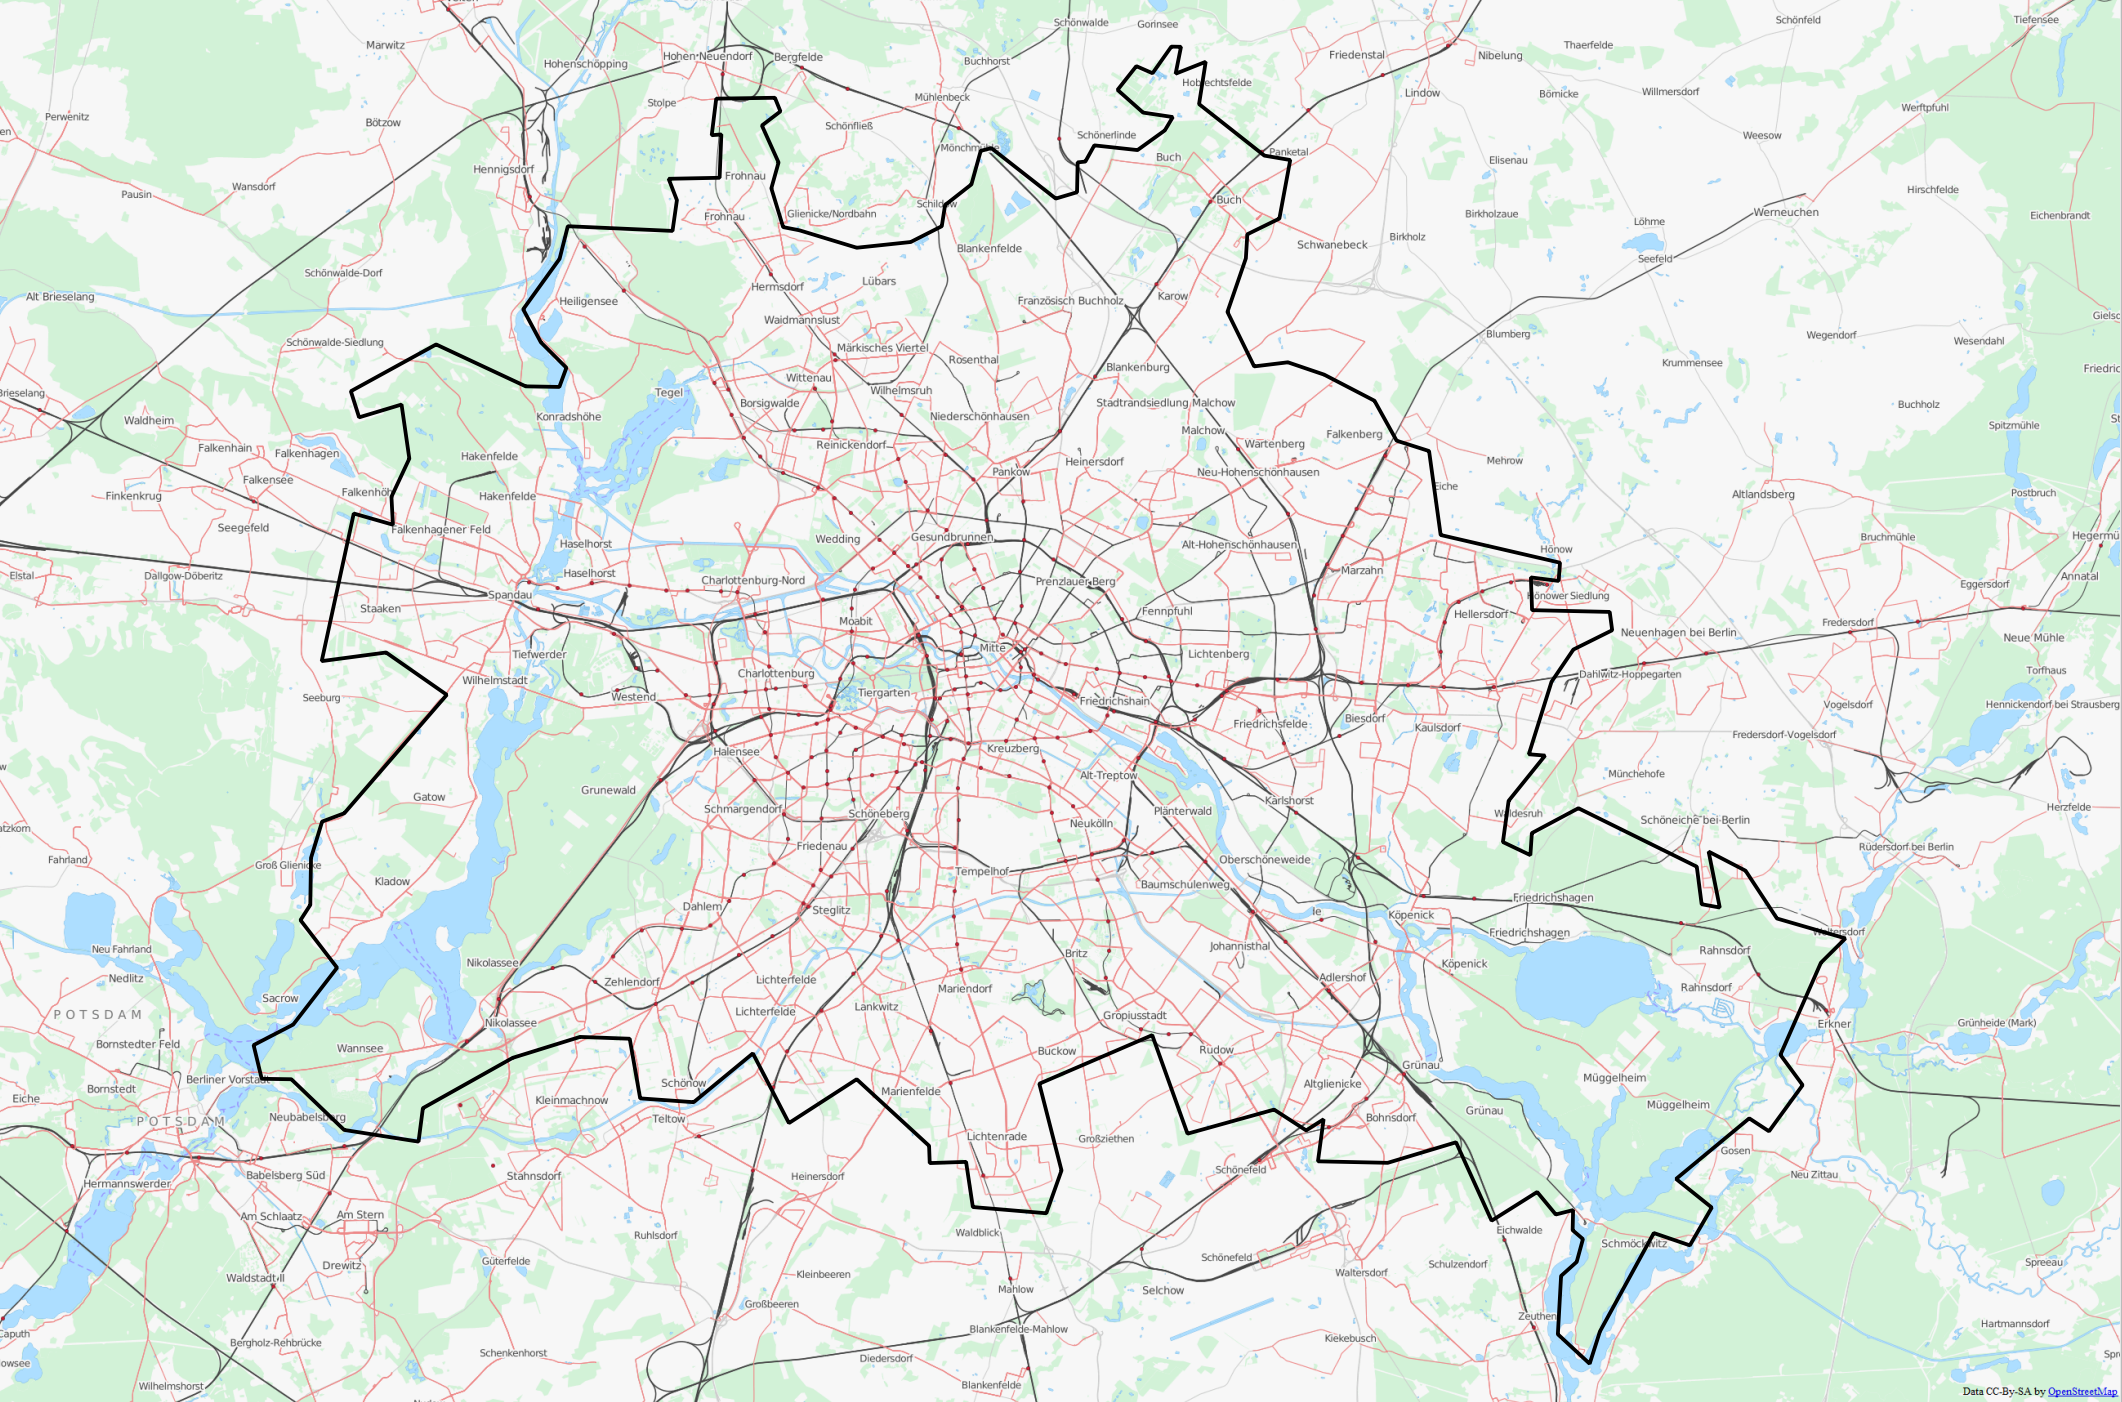
\includegraphics[width=0.99\textwidth, angle=0]{using/figures/berlin_pt}}%
{}
% ------------

% start excerpt from the paper
With the opening of the new Berlin and Brandenburg BER international airport,
Berlin expects major travel demand changes; importantly, the
existing airport Tegel, now exclusively served by \gls{bvg}-operated buses, 
will close. \gls{bvg} thus had substantial interest in a new Berlin area transport model. 
To deal with these changes, the model only had to provide
a base for future regional transport system planning, but also had to supply
detailed information about different user groups' passenger flows. 
Such user group-specific analyses were very important for
the \gls{bvg} in providing a platform for their future business strategies; thus,
an agent-based model was specifically requested. Two scenarios were
required, one for the year 2008 (actual state), and one for the year
2015 (prediction). To meet the above needs, the
\citet{PTV2013} team, \citet{Senozon2013} and \citet{VSP2013} at Technische Universität Berlin (TU Berlin)
offered a combined model consisting of both a static macroscopic model built with
\gls{visum}, as well as an integrated, activity-based demand and
dynamic traffic assignment model, built with \gls{matsim}. During
the project, efforts were made to base both models on the same data
sources and to ensure that both modeling processes interacted with each other to allow data
exchange.
% end excerpt from the paper

To summarize, the model contains about 115\,000 links, % 113269
about 15\,000 directed stops, % 14902
6.0~million agents, % 4422012 (sex) 5992771 (/person)
and 539\,public transport lines operated by \gls{bvg} and other Berlin and Brandenberg state companies. 
Besides motorized individual traffic and public transport, the model also considers biking and walking. 
For a more in-depth description of the model, its generation and its calibration, the reader is referred to the work of
\cite{NeumannEtAl2014IatbrPtBerlinBook}. The model has extensively been used in \citet[][Ch 7/8]{Neumann2014PhD} for the development of the minibus module presented in Section~\ref{sec:paratransit}.

% ##################################################################################################################